\documentclass[12pt,oneside,a4paper]{article}
\usepackage[T1]{fontenc}
\usepackage[utf8]{inputenc}
\usepackage[margin=2.25cm,headheight=26pt,includeheadfoot]{geometry}
\usepackage[danish]{babel}
\usepackage{titlesec}
\usepackage{titling}
\usepackage[framed, numbered]{matlab-prettifier}
\usepackage{changepage}
\usepackage{amsmath}
\usepackage{hyperref}
\usepackage{enumitem}
\usepackage{graphicx}
\usepackage{fancyhdr}
\usepackage{lastpage}
\usepackage{caption}
\usepackage{tocloft}
\usepackage{setspace}
\usepackage{multirow}
\usepackage{float}
\usepackage{comment}
\usepackage{booktabs}
\usepackage{indentfirst}
\usepackage{lscape}
\usepackage[flushleft]{threeparttable}
\usepackage{xcolor}

% --- Danish Translation Fixes ---
\addto\captionsdanish{
  \renewcommand{\contentsname}{Indholdsfortegnelse}
  \renewcommand{\listfigurename}{Liste over figurer}
  \renewcommand{\listtablename}{Liste over tabeller}
  \renewcommand{\abstractname}{Resumé}
  \renewcommand{\refname}{Referencer}
  \renewcommand{\bibname}{Bibliografi}
  \renewcommand{\appendixname}{Appendiks}
  \renewcommand{\indexname}{Indeks}
  \renewcommand{\figurename}{Figur}
  \renewcommand{\tablename}{Tabel}
  \renewcommand{\partname}{Del}
  \renewcommand{\chaptername}{Kapitel}
  \renewcommand{\sectionname}{Afsnit}
  \renewcommand{\subsectionname}{Underafsnit}
  \renewcommand{\authorname}{Forfatter}
  \renewcommand{\date}{\today}
}

% --- Fancyhdr Configuration ---
\pagestyle{fancy}
\fancyhf{}
\setlength{\parindent}{2em}
\renewcommand{\headrulewidth}{1pt}
\renewcommand{\footrulewidth}{1pt}
\lhead{Programmeringsprojekt (30010)\\ Starfighter}
\rhead{\nouppercase{\rightmark}}
\fancyfoot[C]{Side \thepage\ af \pageref{LastPage}}
\setlength\headheight{16pt}
\setlength{\footskip}{50pt}

% --- Code Configurations ---
\usepackage{listings}
\usepackage{color}

\renewcommand{\lstlistingname}{Liste} % Changes "Listing" to "Liste"
\renewcommand{\lstlistlistingname}{Lister} % Changes "List of Listings" to "Lister"

\lstset{
  language=C,
  basicstyle=\ttfamily\small,
  keywordstyle=\color{blue}\bfseries,
  commentstyle=\color{green!60!black},
  stringstyle=\color{red},
  numbers=left,
  numberstyle=\tiny\color{gray},
  stepnumber=1,
  numbersep=8pt,
  showspaces=false,
  showstringspaces=false,
  frame=single,
  breaklines=true,
  captionpos=b
}

\newcommand{\cross}{\ensuremath{\times}}

% --- End of page settings ---



\begin{document}
\pagenumbering{roman} 

\begin{titlepage}
\begin{center}
\vspace{2cm}
%\textsc{ Danmarks Tekniske Universitet}\\[1.5cm]

\includegraphics[width=0.4\textwidth]{root/dtu.png}~\\[1cm]
\vspace{2cm}

\vspace{2cm}

% Title
\hrule
\vspace{.5cm}
{ \huge \bfseries Programmeringsprojekt (30010)\\ Starfighter} % title of the report
\vspace{.5cm}

\hrule
\vspace{1.5cm}

\textsc{\textbf{Forfattere}}\\
\vspace{.5cm}
\centering

% add your name here
Group 08\\
August A. A. Feldthusen - s246569\\
Carl Johann T. B. Falkenhayn - s233318 \\
Jacob J. Olsen - s246048\\
Simon S. Hansen - s246226\\

\vspace{4cm}

\centering \today % Dags dato
\end{center}
\end{titlepage}

\newpage
\doublespacing
\renewcommand{\baselinestretch}{1}\normalsize
\tableofcontents
\renewcommand{\baselinestretch}{1}\normalsize
\thispagestyle{fancy} % force page style


\newpage
\pagenumbering{arabic} 
\fancyfoot[C]{Side \thepage\ af \pageref{EndOfText}}

\newpage
\section*{Resumé} \label{Res}
Dette projekt omhandler udvikling og implementering af et computerspil, der kører på en STM32-mikrocontroller. Spillet er skrevet i programmeringssproget C og er inspireret af det klassiske arkadespil "Space Invaders" med fokus på både funktionalitet og en optimal brugeroplevelse. Projektet benytter desuden en systemarkitektur, som gør mange af spillets komponenter, moduler og funktioner genanvendelige.

Spillet indeholder funktioner som meteorer med tyngdekraft, otte skudvinkler, power-ups samt point og liv vist på en LCD-skærm og kører hurtigt og effektivt. Spillet styres ved hjælp af det eksterne joystick 30010, hvor man både kan bevæge rumskibet, affyre skud og navigere rundt i menuen.

Projektet har givet værdifuld erfaring inden for C-programmering, samarbejde i udviklingsprocessen og softwarearkitektur. Denne rapport dokumenterer design, implementering, udfordringer og resultater og konkluderer, at spillet opfylder kravspecifikationerne, og leverer en unik og god brugeroplevelse. 
\section*{Abstract} \label{Abs}
\input{chapters/Resumé.tex} 

\newpage
\section{Introduktion} \label{ch1}
Formålet med projektet er at designe og implementere et interaktivt arkadespil ved hjælp af en mikrocontroller baseret på en ARM Cortex-M4 CPU og STM32CubeIDE. Projektet fokuserer ikke kun på at skabe et funktionelt og engagerende spil, men også på at overholde industristandarder for spiludvikling. Derudover analyserer projektet et mellemstort programmeringsproblem og håndterer ressourcer og softwarelag på en struktureret og modulær måde.

Spillet, inspireret af det klassiske arkadespil "Space Invaders", indeholder funktioner som meteorer med simuleret tyngdekraft, otte skudvinkler, power-ups vist på en PC-terminal, samtidigt med at point- og livtracking vist på en LCD-skærm. Disse funktioner styres ved hjælp af timere, interrupts og et eksternt joystick. Implementeringens arkitektur består af et applikationslag, applikationsgrænsefladelag og hardwareabstraktionslag, hvilket sikrer god genbrugelighed, så man nemt kan tilføje eller ændre eksisterende funktioner.

Spillet opfylder de obligatoriske krav i projektbeskrivelsen ved at inkludere følgende funktioner: flere kugler, pointtæller, information via RGB-LED, information på LCD-skærmen på en STM32-mikrocontroller, og spillet styres via et eksternt 30010 joystick, der forbindes til mikrocontrolleren. Disse krav er hovedsageligt valgt, ud fra et formål om at genskabe det meget populære arkadespil "Space Invaders".

Ved at følge programmeringsprincipper, såsom minimal brug af globale variabler og modulær kode, sikrer vi præcision og ydeevne, samtidigt med at koden er fokuseret og overskuelig.

Udover at lave et sjovt og funktionelt spil handler projektet også om at lære, hvordan man arbejder med indlejrede systemer og C-programmering. Projektet har også til formål at lære, hvordan man får joystick, RGB-LED'erne og LCD-skærmen til at arbejde sammen. Projektet handler ikke kun om at skrive C-kode – det handler også om at få funktionerne til at fungere på en mikrocontroller med begrænset RAM og ROM.

Denne rapport dokumenterer designovervejelser, implementering og testprocessen for spillet. Rapporten giver indsigt i udfordringer, der blev mødt, og løsninger, der blev implementeret, samt de overordnede resultater af projektet. 

\newpage
\section{Kravspecifikationer} \label{ch2}
\subsection{Minimumskrav}
Spillet skal kunne køre på en STM32-mikrocontroller med begrænset hardware, og systemet skal være robust over for spillerens inputs.\\
Spilleren skal kunne navigere skibet op, ned, til højre og venstre ved hjælp af joysticket samt affyre skud ved at trykke på en knap. Desuden skal spilleren have adgang til en "Boss Key", som skal kunne aktiveres nemt og hurtigt via en af knapperne på joysticket. Spillet skal understøtte flere skudtyper og inkludere tre skydefunktioner: "Laser", "Standard" og "Shotgun", som kan aktiveres af power-ups. Skuddene skal påvirkes af en tilfældig vinkel (random delta). Der skal implementeres kollision mellem skud og fjender, som registreres og fjerner fjenden. Spilleren skal starte med et fast antal liv, som reduceres ved kollision med fjender eller meteorer, eller hvis fjender ikke dræbes, før de rammer skærmens bagside. På den måde er spillerens mål at skyde og eliminere fjenderne, før de forsvinder.\\
Når spilleren mister alle liv, skal spillet afsluttes, og scoren skal vises på LCD-skærmen. Under spillet viser LCD-skærmen spillerens liv, point og den valgte skudtype, hvilket opdateres løbende under spillet.\\
Spillet skal visualiseres i terminalen, hvor skib, skud, fjender og meteorer vises. Teksten "Game Over" skal vises i terminalen, når spillet slutter. RGB-LED'en skal vise antallet af liv tilbage: Grønt lys indikerer tre liv, blåt lys indikerer to liv, og rødt lys indikerer ét liv. LED-skærmen skal slukke, når alle liv er tabt.\\
Koden skal skrives modulært, så nye funktioner som flere fjendetyper eller power-ups nemt kan tilføjes.

\subsection*{Ekstra funktioner}
Der skal tilføjes flere niveauer, der løbende stiger i sværhedsgrad under spillet. I de forskellige niveauer kan spillets sværhedsgrad øges ved at øge fjendernes og meteorernes hastighed eller deres antal. Man kan også gøre fjenderne mindre og meteorerne større, så det bliver udfordrende at ramme fjender, samtidig med at man undviger meteorer. For at undgå at overbelaste mikrocontrolleren er det dog mest hensigtsmæssigt at øge hastigheden på fjender og meteorer fremfor at tilføje flere.

Funktionerne under "\textbf{Minimumskrav}" er prioriterede, fordi de er afgørende for spillets kernefunktionalitet og nødvendige for at gøre det spilbart. Disse funktioner danner fundamentet for spillet og er valgt ud fra deres relevans i forhold til spillets mål og projektbeskrivelsen. Det er vigtigt, at spillet opfylder de grundlæggende krav og er stabilt i sin basisform.

"\textbf{Ekstra funktioner}" inkluderer funktioner, der kan forbedre spiloplevelsen og gøre spillet mere interessant og varieret, men som ikke er nødvendige for, at spillet kan fungere. Disse funktioner kan implementeres løbende, når det essentielle er på plads, og hvis der er tilstrækkelige ressourcer og tid til rådighed.

\begin{itemize}
    \item Systemet skal kunne klare forkerte inputs og fejl i joystick og knapper.
    \item Spilleren skal kunne styre skibet op, ned, til højre og venstre med joysticket.
    \item Spilleren skal kunne affyre skud ved at trykke på en knap.
    \item En "Boss Key" skal kunne aktiveres nemt via en knap på joysticket.
    \item Spillet skal understøtte flere skud-typer "Laser", "Normal", "Shotgun", aktiveret via power-ups.
    \item Skud skal påvirkes af en tilfældig deltavinkel.
    \item Kollision mellem skud og fjender skal registreres og fjenderne fjernes.
    \item Spilleren starter med tre liv, som reduceres ved:
    \begin{itemize}
        \item Kollision med fjender eller meteorer.
        \item Fjender, der undslipper og når skærmens bagside.
    \end{itemize}
    \item Spillet slutter, når spilleren mister alle liv, og scoren vises på LCD-skærmen.
    \item LCD-skærmen viser spillerens liv, point og valgte skud-type, opdateres løbende.
    \item Joysticket skal bruges til skibets bevægelser og menu-navigation.
    \item Koden skal skrives modulært for nemt at kunne tilføje nye funktioner, fjendetyper eller power-ups.
    \item Nye niveauer med stigende sværhedsgrad skal implementeres.
\end{itemize} 

\newpage
\section{Analyse} \label{ch3}
Udviklingen og implementeringen af diverse funktioner er udført i overensstemmelse med blockdiagrammet, der starter med de mest grundlæggende funktioner og udvides derfra.

\subsection{Spiltilstande}
Vores main.c-fil indeholder tre separate spilstadier (\ref{fig:main_flowchart}). Disse er inddelt i tre menuer, som findes i menufolderen under Src-mappen i StarFighter. De tre menuer, der har deres egen fil, står for håndteringen af diverse spilrelevante filer udover initialiseringsfilerne i main.c.\\
Variablen \textit{nav} gives som en pointer i hver spilmenu. Denne variabel opdateres i hver spilmenu afhængigt af spillerens input.
\begin{lstlisting}[caption={Main-løkke kode}]
uint8_t nav = 0;
while (1) {
    if (nav == 0) {
        main_menu(&nav);
    }
    if (nav == 1) {
        help_menu(&nav);
    }
    if (nav == 2) {
        game_menu();
        game_over(&nav);
    }
}
\end{lstlisting}

\subsubsection{Hovedmenu}
Filen \textit{main\_menu.c} indeholder to funktioner. Den ene håndterer al logikken bag hovedmenuen, og den anden bruges til at tegne vinduerne på skærmen. Når spillet initialiseres, sættes \textit{nav} til 0. Dette fører spilleren ind i hovedmenuen.\\
Udover at initialisere hovedmenuens grafik indeholder filen en while-løkke og en integer, \textit{z}. Variablen \textit{z} opdateres i while-løkken afhængigt af funktionen read\_joystick, som aflæser positionen af 30010-joysticket i realtid. Variablen \textit{z} styrer også de visuelle input, der hjælper spilleren med at indikere, hvilken menu der vælges.\\
Derudover indeholder while-løkken to if-sætninger, der tjekker værdien af \textit{z} og inputtet fra read\_button, som er en funktion fra joystick\_reader.c. Kombinationen af disse to afgør, hvad \textit{nav} sættes til, og dermed hvilken menu spilleren føres ind i.

\subsubsection{Spilmenu}
Filen \textit{game\_menu.c} indeholder to funktioner: Funktionen \textit{game\_menu()} indeholder al initialisering, der er relevant for spilstyring, grafik og andre elementer. Derudover indeholder den en while-løkke, der opdaterer alt fra kollisionsmekanik til LCD-skærmen. Denne while-løkke brydes først, når spillerens liv når nul. Herefter initialiseres funktionen \textit{game\_over()}, der bruger pointeren \textit{nav}.\\
Funktionen game\_over har sin egen while-løkke, der tjekker for input fra joysticket og sender spilleren tilbage til hovedmenuen.

\subsubsection{Hjælpemenu}
Filen \textit{help\_menu.c} indeholder en af de tre menuskærme, der bringer spilleren rundt i spillet. Den indeholder en funktion, der bruger variablen \textit{nav} til at tegne skærmens grafik samt en while-løkke, der tjekker, om knap ét eller to trykkes.\\
Variablen \textit{nav} angiver en værdi: 0, 1 eller 2, som angiver, hvilken af de tre menuer den skal gå ind i. Herefter bliver man sendt tilbage til hovedmenuen.

\subsubsection{Boss-key/Pauseskærm}
Filen boss\_key.c indeholder opsætningen af funktionen \textit{boss\_key()}. Funktionen indeholder en if-sætning, der evalueres hver gang game-while-løkken kører. Dette kan ses i game\_menu.c.\\
Funktionen sætter den globale variabel \textit{cs}, som er spillets timer, på pause. Dette forhindrer spillerens point i at stige, og positionerne af aliens, meteorer og skud ændres ikke. Herefter vises boss-key-skærmen og går ind i en while-løkke, hvor den afventer input fra "knap to". Dette genstarter timeren \textit{cs} og game-løkken, så alt fortsætter fra dér, hvor man var nået til.\\
Grafikken er udarbejdet ved hjælp af forskellige ASCII-relevante hjemmesider: \cite{Text_to_ASCII_converter} \cite{ASCII_art}.


\subsection{Skud}
\subsubsection{Skudstruktur}
Skuddets struktur indeholder position, hastighed, hvorvidt skuddet er ”aktivt” eller ej, samt om det er blevet påvirket af tyngdekraft. Disse oplysninger bruges til at håndtere og opdatere skuddets position. Hvis et skud er aktivt, opdateres skuddets position jævnligt ved at addere med hastigheden.
\begin{lstlisting}[caption={Skudarray kode}] 
typedef struct {
    uint8_t bx;
    uint8_t by;
    int8_t vx;
    int8_t vy;
    uint8_t active;
    uint8_t gravity;
} bullet;
\end{lstlisting}

\subsubsection{Skudvinkler}
Rumskibet har en variabel, der registrerer den seneste retning, som rumskibet har bevæget sig i (\textit{pos->direction}). Variablen kan have en værdi fra \(1\) til \(8\), som angives af \textit{read\_joystick()}.\\
Når rumskibet skyder, indstilles skuddets hastighedsvektor ud fra retningsvariablen. Hvis rumskibet for eksempel peger mod højre, sættes hastigheden langs \(x\)-aksen til \(2\) og langs \(y\)-aksen til \(0\). Hvis rumskibet peger skråt ned mod venstre, sættes hastigheden langs \(x\)-aksen til \(-2\) og langs \(y\)-aksen til \(1\).\\
Eftersom pixlerne fylder dobbelt så meget på \(y\)-aksen som på \(x\)-aksen, er det nødvendigt at fordoble hastigheden langs \(x\)-aksen i forhold til \(y\)-aksen, så alle retninger føles lige hurtige.

\subsubsection{Håndtering af flere skud}
Muligheden for at affyre flere skud er implementeret ved hjælp af et array. Når spillet startes, oprettes et array, hvor størrelsen er det maksimale antal skud, der kan eksistere samtidigt. Derefter opdateres skuddenes positioner ved at iterere over arrayet og udføre de nødvendige beregninger.\\
For at sikre jævne opdateringer opdateres skuddene forskudt af hinanden baseret på deres indeks.
\begin{lstlisting}[caption={Skudarray kode}] 
bullet bullets_array[MAX_BULLETS];
\end{lstlisting}

\subsubsection{Kollisionsregistrering}
Kollisionsregistrering udføres ved at sammenligne positioner med if-sætninger. Da objekternes positioner i spillet (rumskibet, skud, aliens, meteorer) er placeret i det øvre venstre hjørne af objektet, håndteres skudkollision med meteorer som følger:\\
Hvis skuddets \(x\)-værdi er større end meteorens \(x\)-værdi og mindre end meteorens \(x\)-værdi plus 20, og skuddets \(y\)-værdi er større end meteorens \(y\)-værdi og mindre end meteorens \(y\)-værdi plus 10, udføres udsagnet indeni. I dette tilfælde fjernes skuddet.
\begin{lstlisting}[caption={Kollisionsregistrering kode}]
for (uint8_t i = 0; i < MAX_BULLETS; i++) {
    for (uint8_t j = 0; j < MAX_METEORS; j++) {
        if ((bullets_array[i].bx >= meteors_array[j].x)
            && (bullets_array[i].bx < meteors_array[j].x + 20)
            && (bullets_array[i].by >= meteors_array[j].y)
            && (bullets_array[i].by < meteors_array[j].y + 10)) {
            bullets_array[i].active = 0;
        }
    }
}
\end{lstlisting}

\subsubsection{Tyngdekraftseffekt}
Tyngdefeltet omkring meteorerne er implementeret på en simpel, men effektiv måde. Det fungerer ved at tjekke, om et skud passerer forbi en meteor inden for en rækkevidde. Hvis det gør, afbøjes skuddet ved at ændre dets hastighedsvektor.\\
Selvom det ikke er fysisk realistisk, fungerer det godt i spillet, da det er let for computeren at beregne og forudsigeligt for spilleren.\\
Derudover indeholder skuddets struktur en variabel, der registrerer, om skuddet er blevet påvirket af tyngdekraft, så det ikke afbøjes flere gange.
\begin{lstlisting}[caption={Tyngdekraftseffekt kode}]
for (uint8_t i = 0; i < MAX_BULLETS; i++) {
    if (bullets_array[i].gravity == 0) {
        for (uint8_t j = 0; j < MAX_METEORS; j++) {
            if ((bullets_array[i].bx >= meteors_array[j].x - 20) &&
                (bullets_array[i].bx <= meteors_array[j].x) &&
                (bullets_array[i].by == meteors_array[j].y + 5)) {
                
                bullets_array[i].vx++;
                bullets_array[i].gravity = 1;
            }
        }
    }
}
\end{lstlisting}

\subsubsection{Skudtyper}
Implementeringen af nye skudtyper er meget ligetil, når skudfunktionaliteten allerede er opsat.\\
Vores "shotgun" er implementeret ved, at rumskibets retning drejes én gang mod venstre, idet der skydes. Derefter drejes rumskibet én gang mod højre og skyder igen, hvorefter det drejes tilbage og skyder en sidste gang. Dette sker så hurtigt, at spilleren ikke bemærker, at rumskibet drejer og skyder gentagne gange. Resultatet er, at rumskibet praktisk og visuelt skyder tre spredte skud.\\
Laseren er implementeret anderledes, da programmet undersøger, om der er aliens foran rumskibet, når skuddet affyres. Hvis der er, elimineres de. Derefter vises et blink af en hvid streg på skærmen for at kommunikere visuelt til spilleren, at laseren er blevet affyret.

\subsection{Fjender}
\subsubsection{Fjendefrembringelse}
Meteorer og aliens fremkaldes på stort set samme måde: Først tjekkes det, om fjendenummer \(i\) er aktiv. Hvis den ikke er aktiv, sættes dens \(x\)-koordinat til 243, hvilket er den maksimale \(x\)-værdi. Derefter bestemmes dens \(y\)-koordinat "tilfældigt" ved at beregne:
\[
cs \bmod \left( (\text{højden af skærmen} - 2) - \text{højden af fjenden} \right) + 1.
\]
Dette sikrer, at fjenden ikke genereres for højt eller for lavt, samtidig med at det føles tilfældigt for spilleren. Fjenden sættes derefter til at være aktiv. Når en fjende er aktiv, bevæger den sig mod venstre, og man tager skade af at ramme den med rumskibet.

\subsubsection{Fjendebevægelse}
Fjender bevæges ved først at slette den bagerste række af deres grafik, hvorefter deres nye position beregnes. Hvis en fjendes nye position er uden for skærmen, sættes fjenden til at være inaktiv, og spilleren mister et liv. Hvis ikke, printes fronten af modstanderen. På denne måde bevæger fjenderne sig glat hen over skærmen ved simple operationer.

\subsubsection{Stigende alienhastighed ved timer}
Når runden starter, sættes alienes bevægelseshastighed til \(15\). Derefter stiger deres bevægelseshastighed gradvist gennem spillet for at øge sværhedsgraden. Dette implementeres ved at ændre deres opdateringsinterval.
Al bevægelse i spillet fungerer via opdateringer, hvor hyppigheden af opdateringerne bestemmer bevægelsens hastighed. Derfor nedsættes alienes opdateringsinterval gradvist gennem spillet.
\begin{lstlisting}[caption={Stigende alienhastighed kode}]
if (cs % 2500 == 0) {
    alien_speed--;
}
\end{lstlisting}

\subsubsection{Forsinkelser}
Der er indsatte forsinkelser flere steder i koden for at undgå, at funktioner kaldes for ofte. Dette implementeres ved at sætte en variabel (for eksempel \textit{last\_fire\_time}) til værdien af \textit{cs}, når funktionen kaldes. Næste gang funktionen så kaldes, tjekkes det, om forsinkelsen siden sidste kald er tilstrækkelig til, at funktionen kan kaldes igen.\\
Dette kan for eksempel ses i funktionerne \textit{fire\_bullet()} og \textit{spawn\_alien()}:
\begin{lstlisting}[caption={Forsinkelse kode}]
if (cs - last_fire_time < BULLET_FIRE_DELAY) {
    return;
}
last_fire_time = cs;
\end{lstlisting}

\subsection{LCD}
\subsubsection{LCD-skærmens opbygning}
Vores Liquid-crystal display (LCD) bruges til at vise spillerens liv, point og hvilken skudtype spilleren har aktiveret. Displayet er opdelt i 512 byte, som yderligere er inddelt i 4 rækker med 128 byte hver.\\
Displayet fungerer ved, at en usigneret 8-bit buffer med 512 bytes hukommelse (\textit{uint8\_t lcd\_buffer[512]}) modtager start-inputtet og ved hjælp af binære tal (omskrevet til hexa-decimaler) angiver, hvad den givne byte skal vise. For eksempel skrives hexadecimalen \textit{0xF7} som \textit{1111 0111} i binært og vil blive vist som en streg, hvor "1"-tallene svarer til tændte (mørke) felter på displayet. Ved at ændre hexadecimale værdier og startpositionen kan funktionen bruges til at tegne statiske figurer, som for eksempel hjerter, tekst eller omridset af den valgte skydetilstand.\\
For at aktivere displayet skal displayet først initialiseres ved hjælp af funktionen \textit{lcd\_init()}. Derefter bruges \textit{memset(lcd\_buffer, 0x00, 512)} til at nulstille alle 512 bytes i displayet for at undgå ”gryn” på skærmen. Til sidst uploades de ønskede data til displayet ved hjælp af funktionen \textit{lcd\_push\_buffer(lcd\_buffer)}.

\subsubsection{Liv}
Liv visualiseres med tre hjerter i det øverste venstre hjørne, som opdateres i realtid, når spilleren mister liv i spillet. Funktionen \textit{hearts()} tager en startposition som input og tegner et enkelt hjerte på displayet. Her angiver startpositionen, hvor på displayet hjertet skal placeres. Funktionen benytter en række buffere til at udfylde hjertet kolonne for kolonne. Til sidst holder funktionen \textit{hearts\_left()} styr på antallet af tilbageværende liv og opdaterer displayet med tilføjelse eller fjernelse af hjerter.

\subsubsection{Tekst}
For at skrive tekst som liv og point på displayet har vi oprettet funktionen \textit{lcd\_write\_string}. Den tager en streng og en startposition som input, og så gennemløber while-løkke strengen karakter for karakter og fortsætter udskrivningsprocessen, så længe strengen ikke er nul. \textit{uint8\_t c = *str++} læser den enkelte karakter i strengen, gemmer den i variablen \textit{c} og går derefter videre til næste karakter. Der trækkes 32 fra \textit{c}, da ASCII-tabellen i \textit{charset.c/h} giver bogstaver fra plads 32.\\
En for-løkke sørger for at udskrive hver karakter – i dette tilfælde bogstaver – én pixelkolonne ad gangen. Karaktererne genereres ud fra \textit{character\_data}, som er et array i \textit{charset.c}, hvor pixelopbygningen af hver karakter er defineret pixelkolonne for pixelkolonne. Karaktererne er 5 pixelkolonner brede.

\subsubsection{Skud tilstand}
Funktionen \textit{shooting\_mode\_box()} kommunikerer med den aktuelt aktiverede skudtype via en struktur. Ved at forbinde opsætningen af funktionen \textit{heart()} med if-sætninger kan displayet skifte mellem de tre viste skudtyper. Den samme opsætning bruges i \textit{remove\_shooting\_mode\_box()} til at fjerne gamle linjer, når skudtypen ændres.

\subsubsection{Pointsystem}
De point, som vises på LCD-skærmen, er knyttet til timeren \textit{cs}. LCD-skærmen opdateres kun, mens spillet er i gang. Når spilleren dør, stopper timeren. Når spillet genstartes, nulstilles timeren (\textit{cs}) til 0, hvilket også nulstiller pointene.

\subsubsection{RGB-LED}
LED-skærmen på STM32-mikrocontrolleren styres af variablen \textit{health}. Når \textit{health} er 3, lyser LED’en grønt. Ved 2 liv lyser den blåt, og når der kun er 1 liv tilbage, lyser den rødt. Dette implementeres med en funktion, der tager tre binære inputs (\textit{R}, \textit{G} og \textit{B}) og konverterer dem til værdier, som sendes til LED-skærmens GPIO-port. 

\newpage
\section{Design} \label{ch4}
\subsection{Kvalitetssikring}
Kvalitetssikring er en central del af projektet for at sikre, at spillet fungerer stabilt og opfylder alle krav. For at opnå dette har vi implementeret flere strategier til at teste systemets funktionalitet og sikre robustheden af vores kode.\\
Sideløbende med udviklingen af de individuelle moduler har vi testet dem hyppigt for at sikre, at de fungerer som forventet. Der opstår ofte problemer, når modulerne implementeres i en main-løkke, men disse er lettere at løse, hvis de individuelle dele allerede er verificeret.\\
Når vi støder på udfordringer med at finde fejl i koden, bruger vi debuggingværktøjerne, der er en del af STM32CubeIDE. Denne tilgang hjælper os med at finde og rette logiske fejl samt løse kommunikationsproblemer mellem softwarelagene.

\subsection{Hardware- og tidsmæssige begrænsninger}
En af de største udfordringer ved dette projekt er at arbejde inden for de begrænsninger, som STM32-mikrocontrolleren stiller. Selvom STM32-platformen er meget alsidig, udgør den stadig en væsentlig begrænsning ift. RAM og ROM. Dette betyder, at vi konstant skal overveje, hvordan vi udnytter de ressourcer, den stiller til rådighed.
Spillets funktioner skal være optimeret, så spillet kører gnidningsfrit og optimalt, uden at overbelaste mikrocontrolleren. Derudover skal antallet af globale variabler være minimeret, og der sikres, at vores funktioner kun bruger de nødvendige ressourcer.\\
Med kun to uger til rådighed har det tidsmæssige pres gjordt det nødvendigt at balancere mellem design, implementering og test af spillet, hvilket har krævet en stram tidsplan og klare prioriteringer. De essentielle funktioner er prioriteret først – såsom joystickstyring, kollision og skudmekanik – før vi tilføjede avancerede funktioner som "power-ups" og RGB-indikatorer. Grundet den faste tidsramme, skaber prioriteringen en buffer, som i tilfælde af at tidsplanen skubbes, stadig efterlader os med et funktionelt spil.\\

Spillet indeholder en global varibel, hvilket er \textit{cs}. Den er implimenteret for at holde styr på alle vores variabler. Den kaldes hver gang, der bliver lavet interupt af den indbyggede timer i mikrocontrolleren, hvilken øger dens værdi med én.
\begin{lstlisting}[caption={Timer kode}]
void TIM1_BRK_TIM15_IRQHandler(void) {
    cs++;
    TIM15->SR &= ~0x0001; // Clear interrupt bit
}
\end{lstlisting}



\subsection{Grafisk design}
Det grafisk design er lavet med ASCII-tegn, da det grundet tidligere erfaringer har vidst sig at være en nem og tilstrækkelig måde at opbygge spillet på. Grundet tekniske forskelle i størrelse af computer/laptop skærme, blev terminalens opløsning bestemt til 243x76 pixels. Dette er med til at sikre at spillet kan køres optimalt på samtlige computerer og give den sammen bruger oplevelse, uden yderligere visuelle begrænsninger.\\


Dette gør det muligt at prioritere gameplay og funktionelle krav uden at introducere unødvendige kompatibilitetsproblemer forårsaget af skift i opløsningen. Derudover gør dette det muligt at "hard-code" vores grafik til præcist denne opløsning.\\
Generelt blev avanceret grafik nedprioriteret gennem forløbet af to årsager: Den første er fordi det er meget ensformigt og tidskrævende at kode store figurer med ASCII-tegn. Den anden skyldes problemer med opdatering af terminalen, da samtlige objekter på skærmen blev hhv. slettet og genprintet for at skabe følelsen af at de bevægede sig. Simplerer figurer og karakterer er derfor foretrukket grundet, at de er lettere at manipulerer med. Det simple udtryk passer også godt til det overordnede "Space Invaders"-tema.

\subsubsection{Grafikkens bevægelse}
Vi afprøvede forskellige metoder til at optimere animationen af grafikken, blandt andet ved at øge Baud-raten, som påvirker print-hastigheden i terminalen. Vi startede med en Baud-rate på 9600, men opdagede hurtigt, at bevægelser i terminalen (fx et skud, der flyttede sig) var meget langsomme og forsinkede. Derfor undersøgte vi muligheden for at øge Baud-raten og opdagede, at \(115.200\) fungerede godt. Denne hastighed kunne håndtere mere bevægelse, så længe der kun var én bevægende del ad gangen.\\
Da vi begyndte at introducere større figurer og grafik, der skulle bevæge sig over baggrunden, blev det dog tydeligt, at dette ikke var tilstrækkeligt.I den konfiguration, vi brugte, anvendte vi en \textit{clrscr}-funktion, som ryddede hele skærmen og derefter tegnede baggrunden og den opdaterede grafik. Denne tilgang var for tidskrævende og skabte forstyrrelser i den jævne overgang mellem grafikkens positioner.\\
For at løse dette optimerede vi baggrundsfunktionen \textit{init\_baggrund}, så den nu tager fire parametre, der repræsenterer koordinaterne for hjørnerne af en firkant. Dette gør det muligt kun at opdatere de baggrundsdele, der bliver påvirket af bevægelsen. Derudover udviklede vi en ny funktion til at rydde skærmen selektivt, så kun de relevante dele af grafikken blev fjernet. Både aliens og meteorer bevægede sig meget forudsigeligt, hvilket gjorde det oplagt kun at slette og tegne de relevante dele af dem ved opdatering af deres bevægelse.\\
En anden vigtig optimering, vi implementerede, var at skifte fra if-sætninger til switch-sætninger flere steder i koden, der håndterer objekters bevægelser og handlinger. Ved at anvende switch-sætninger reducerede vi kompleksiteten og forbedrede læsbarheden af koden, samtidig med at vi optimerede dens ydeevne. Dette skyldes, at switch-sætninger er mere effektive til at håndtere flere mulige cases sammenlignet med lange kæder af if-else-sætninger, især når mange scenarier skal behandles.\\
Disse forbedringer resulterede i en mere jævn og effektiv opdatering af baggrunden og grafikken. Selvom disse ændringer fik spillet til at køre tilfredsstillende, valgte vi at øge Baud-raten til \(345.600\), hvilket på vores computere var den maksimale hastighed uden tilfældige fejl. Dette resulterede i, at spillet kørte både bedre og hurtigere, hvilket markant forbedrede spiloplevelsen.

\subsection{System abstraktionslag}
Vi anvender en lagdelt struktur i vores projekt. Dette sikrer både en tydelig struktur og høj effektivitet i vores arbejde. Denne struktur hjælper os med at holde styr på prioriteringerne, da funktionaliteten i Hardware Abstraction Layer (HAL) skal være på plads, før elementer i Application Layer kan fungere. I det følgende beskrives de tre lag, samt hvilke filer der indgår i projektet, og hvad deres funktion er.

\subsubsection{Application layer}
Til vores application layer opretter vi en mappe kaldet "graphics". Her placerer vi alt spilgrafik, bortset fra de forskellige spil-menuer og boss-key, som også indeholder noget grafik.\\
Det første, vi udvikler i "graphics"-mappen, er baggrunden. Vi starter med funktionen \textit{bigplanet}, som tegner en planet med to farver på en given position. Oprindeligt ønskede vi at bruge planeter som baggrund under spillet, men det krævede for mange ressourcer at gentegne dem, når noget bevægede sig over dem. Derfor valgte vi at bruge planeterne udelukkende i menuen \textit{game\_start}, hvor gentegning ikke var nødvendig.\\
Til baggrunden tilføjede vi \textit{stars}, som placerede "*" forskellige steder på skærmen for at simulere stjerner. Selvom vi overvejede at bruge en funktion til at generere deres placeringer tilfældigt, valgte vi i sidste ende at hardkode deres positioner. For det første er det mere effektivt for mikrocontrolleren at arbejde med hardcodede positioner, og for det andet er det nemmere at genskabe baggrunden, når stjernernes placering kendes præcist. Ulempen ved denne tilgang er, at hardcodning gør funktionen mindre genanvendelig.
Da vi startede med to funktioner (\textit{big\_planet} og \textit{stars}), udviklede vi også \textit{init\_background}, som skulle kombinere disse funktioner til én samlet baggrund. I praksis endte \textit{init\_background} dog med kun at kalde \textit{stars}-funktionen.
\newline
\textbf{Enemy}
\newline
Til fjender starter vi med at fastlægge grafikken. Vi vælger en simpel grafik, da den skal bevæge sig og opdateres ofte.

Funktionen \textit{Init\_enemy\_state} initialiserer fjenderne ved at sætte alle elementer i både \textit{aliens\_array} og \textit{meteors\_array} til inaktive.

Når der findes en inaktiv meteor, sørger \textit{spawn\_meteor} for at placere den i højre side af skærmen og sætte den til aktiv. \textit{Spawn\_alien} fungerer lidt anderledes, da den også tjekker, hvor lang tid der er gået siden den sidste alien blev spawnet, før en ny alien skabes.

I funktionen \textit{enemy\_go} opdateres både meteorer og aliens. Meteorer genereres, flyttes mod venstre på skærmen og opdateres. For aliens sker det samme, men deres grafik gør processen en smule mere kompleks.
\newline
\textbf{Powerup}
\newline
I \textit{powerup} er der kun 2 funktioner: \textit{powerup} og drawwindow. \textit{Drawwindow} funktionen tegner et 16x8 vindue med en bestemt farve. Vinduet bliver lavet med ASCII-karakterer. I \textit{powerup} tegnes vinduet fra \textit{drawwindow} og midten af dette beregnes. Funktionen tager så nogle cases alt efter hvilken powerup der skal tegnes. Her har vi 3: Laser, hjerte og shotgun.
\newline
\textbf{Spaceship}
\newline
Da vi udvikler grafikken til rumskibet, beslutter vi, at det skal kunne dreje i fire retninger. Derfor skaber vi fire forskellige grafikker til rumskibet. Ideelt set ville vi gerne have haft otte retninger, så det kunne dække alle bevægelsesretninger, men vi støder på begrænsninger med ASCII-tegn, da det er svært at designe et rumskib, der eksempelvis peger 45 grader opad.

Vi laver to forskellige designs: ét, der håndterer retningen opad, og ét, der peger mod højre. Disse designs inverterer vi for at dække alle fire retninger. De fire grafikker samles i funktionen \textit{draw\_spaceship}, som tegner én af de fire mulige orienteringer baseret på dens parameter.
\newline

\subsubsection{Application interface layer}
\textbf{ANSI}
\newline
I graphics-mappen findes vores ansi-fil, der giver adgang til ANSI escape-sekvenser. Disse sekvenser gør det muligt at skrive funktioner som \textit{fgcolor}, der sætter forgrundsfarven for teksten i terminalen, \textit{bgcolor}, der sætter baggrundsfarven, og \textit{resetbgcolor}, der nulstiller farverne.

Ansi-filen bruger ASCII-tegn, så eksempelvis vil \textit{fgcolor(6)} sætte forgrundsfarven til cyan.
\newline
\textbf{LCD}
\newline
LCD'ens funktion er at fremvise spillerens liv, point samt hvilken \textit{bullet-type} spilleren har aktiveret. Livet er visualiseret med tre hjerter i topvenstre hjørne, som opdateres i realtid med at spilleren mister liv i spillet. Funktionen \textit{hearts} tager en startsposition som input og printer et enkelt hjerte. Startspositionen er baseret på, hvor på LCD-skærmen vi ønsker at placere hjertet. LCD-skærmen er opdelt i 512 bytefelter, som yderligere er opdelt i 4 rækker med hhv. 128 byte felter i hver.  Displayet fungerer ved at 


\subsubsection{Hardware abstraction layer}

\textbf{30010 joystick}\\
30010-joysticket blev sat op efter \textit{Assignment 8} i kurset 30010 på DTU \cite{lecture_notes_uge_2}. Under \textit{joystick\_reader.c} i funktionen\textit{ configure\_adv\_joystick} kan det ses, at ADC1 bruges til at konvertere det analoge signal til et digitalt. Pin C2 og C3 bliver brugt til at modtage joystickpositionen. For at aflæse joystickets \(x\)- og \(y\)-koordinat bruges channel 8 og 9 som der bruges til vores pinopsætning\cite{Reference_Manual_RM0365}. De to funktioner read\_adv\_joystick\_x og -y returnerer værdien fra joystickens to akser. Disse to funktioner bliver videre brugt til kategorisering af joystickens retning som kan ses under funktionen read\_joystick Pin C10 og C12 bliver brugt til at aflæse de to knappers input. Alle fire pins bliver sat til pull-down registre der måler en spændingsforskel når de bliver trykket. 

\newpage
\section{Projektet} \label{ch5}
\subsection{GitHub}
Til dette projekt brugte vi GitHub til samarbejde og fildeling. GitHub hjalp os med at organisere projektets filer, holde styr på ændringer og arbejde på forskellige dele af koden parallelt uden at risikere store konflikter. Desuden gjorde det fildeling nemmere og hjalp med at undgå, at det blev rodet.\\
Repositoryet var struktureret med en main-branch til stabile versioner og separate branches til hvert gruppemedlem for at holde main-branchen stabil. Brugen af GitHub og versionskontrol gjorde ikke kun projektarbejdet mere struktureret, men lærte os også vigtige principper for samarbejde og dokumentation i softwareudvikling.

\subsubsection{Tidsstyring og prioritering}
For at prioritere vores tid bedst muligt lavede vi både en dag-for-dag tidsplan og et GANTT-diagram for at sikre et godt overblik over vores tid. Planen blev opfattet som dynamisk og brugt som en guideline, da ændringer kunne ske dagligt. Det vigtigste udbytte af tidsplanen var at planlægge, hvordan vi skulle arbejde sammen. Det var vigtigt, at vi havde de samme prioriteringer for, hvad der var vigtigt for spillet, og sikrede, at funktionerne blev implementeret og testet i en logisk rækkefølge. Vi begyndte med at programmere spillets "need to haves" og tilføjede derefter eventuelle "nice to haves".

\subsection{Projektverificering}
Under udviklingen af spillet stødte vi på flere udfordringer og fejl, som krævede systematisk debugging for at sikre stabilitet og korrekt funktionalitet. En af de mest almindelige udfordringer var fejl i kommunikationen mellem lagene i vores program, som ofte skyldtes enten forkert initialisering af GPIO'er og timere eller fejl i logikken i vores kode.\\
For at identificere og rette logiske fejl anvendte vi forskellige debugging-teknikker, herunder breakpoints i STM32CubeIDE med variabelvisning og serielle udskrifter til terminalen. Dette gjorde det muligt at kontrollere og verificere værdierne af variabler og signaler i realtid. 

\newpage
\section{Brugermanual} \label{ch6}

\subsection{Putty konfiguration}
Sæt '\textit{Connection type}' til '\textit{Serial}' og '\textit{Serial line}' til den pågældende indgang MCU'en er tilsluttet til. Baudrate sættes til 345.600.

\subsection{Spilstyring}
Brug 30010-joysticket til at navigere rundt i menuerne, og brug B1 og B2 til at navigere ind i menuerne. Hjælp-menuen giver et kort resumé af spillet og dets udfordringer. Start-knappen initialiserer spillet, og du spawner  til venstre i midten af skærmen.\\
LCD-skærmen aktiveres herefter, og du kan se både antallet af liv (også indikeret af LED’en) og din aktuelle score. Brug B2 til at skyde med den valgte ammunition. B1 aktiverer boss-key, som pauser din score. Et tryk på B2 bringer dig tilbage til spillet, præcis hvor du slap, før boss-key blev aktiveret.\\
Du mister et liv, hvis du rammer en alien, eller hvis en alien når den venstre side af skærmen. En kollision mellem dit skib og en meteor dør du af. Power-ups aktiveres automatisk ved kollision med dem.\\
Der findes tre power-ups, hver med deres unikke ikon: Shotgun, laser og heal. Shotgun affyrer tre skud ad gangen i hver sin retning. Laser affyrer en stråle, der kan trænge igennem både aliens og meteorer, og heal giver spilleren et ekstra liv. LCD’en indikerer, hvilken af de tre ammunitionstyper spilleren er udstyret med.\\
Når spilleren mister alle sine liv, stopper spillet, og 'GAME OVER' vises på skærmen. Spilleren kan nu aflæse sin endelige score på LCD’en. Et tryk på en af knapperne sender spilleren tilbage til menuen, hvor spillet kan startes forfra.

\subsection{\textbf{Pinopsætning}}
\begin{itemize}
    \item ADC1 -> PC\_3 
    \item ADC2 -> PC\_2
    \item GND -> GND 
    \item VDD -> 3V3
    \item B1 -> PC\_12
    \item B2 -> PC\_10
\end{itemize} 

\newpage
\section{Diskussion} \label{ch7}
\subsection{Projektets styrker og svagheder}
\subsubsection{Styrker}
En af projektets største styrker er den modulære arkitektur, som udgør fundamentet for projektets design. Den modulære tilgang gør det muligt at arbejde parallelt på forskellige moduler og samle dem senere. Konsekvent spiltestning og debugging sikrer, at større bugs og problemer undgås senere i udviklingsprocessen.\\
Derudover indeholder projektet en række avancerede funktioner og udnytter mange af de indbyggede egenskaber i STM32CubeIDE, såsom LCD-skærmen. Dette forbedrer både brugerens spiloplevelse og gør spillet mere unikt.

\subsubsection{Svagheder}
En af de største udfordringer er projektets tidsbegrænsninger: Man skal både lære C og udvikle et spil på blot tre uger. Selvom man har en klar plan, kan nogle opgaver vise sig at være væsentligt mere tidskrævende, end man oprindeligt forudser. Dette kan føre til, at man uforudset må nedprioritere funktioner, der forbedrer spilleoplevelsen, for i stedet at fokusere på de grundlæggende funktioner.\\
Det komplekse miljø i STM32CubeIDE er desuden svært at navigere for begyndere i C. Der opstår mange udfordringer, når man skal forstå den omfattende brugermanual på over 1000 sider og samtidig håndtere maskinens skavanker. Desuden har forskellige programmører ofte forskellige skrivestile, og uden en klart aftalt navngivningskonvention for filer og funktioner kan det skabe problemer.\\
Alt dette kan skabe udfordringer under implementeringen af koden, men det er stadig overkommeligt. Vi aftalte for eksempel tidligt at bruge snake_case og sørgede for at implementere det konsekvent undervejs.

\subsection{Joystick-implementering}
Ved implementeringen af 30010-joysticket stødte vi på flere problemer. Med et analogt signal på 12 bits ville man forvente, at den læste en signalstyrke mellem 0 og 4095. Vi målte dog værdier mellem 750 og 3500 med mindre variation mellem joystickets \(x\)- og \(y\)-akse.\\
Dette resulterede i, at if-sætningerne blev konfigureret baseret på vores målinger. Disse if-sætninger ville ikke fungere korrekt, hvis 30010-joysticket virkede normalt.\\
I appendix findes kode til brug med et normalt fungerende joystick (\ref{kode:If-sætninger til normalt fungerende 30010 joystick}). Denne kode skal indsættes i if-sætningerne i funktionen \textit{read\_joystick()} i filen \textit{joystick\_reader.c}, som findes i mappen \textit{init}.

\subsection{Krav}
\begin{itemize}
    \item Systemet skal kunne klare forkerte inputs og fejl i joystick og knapper.
\end{itemize}
Systemet reagerer ikke på ugyldige inputs, og dermed er dette ikke et problem. Hvis man for eksempel er i "Help Menu", og klikker på den hvide knap, sker der ingenting.

\begin{itemize}
    \item Spilleren skal kunne styre skibet op, ned, til højre og venstre med joysticket.
\end{itemize}
I spillet kan man styre skibet i otte retninger, dog kan grafikken kun vise fire retninger. Det sker, da grafikken er lavet med ASCII-karakterer, og vi konluderede, at et diagonalt rumskib ikke kan eksekveres pænt.

\begin{itemize}
    \item Spilleren skal kunne affyre skud ved at trykke på en knap.
\end{itemize}
Man kan skyde i 8 forskellige retninger. Det kræver dog meget processorkraft i mikrocontrolleren, hvilket resulterer i, at man må begrænse antallet af skud.

\begin{itemize}
    \item En "Boss Key" skal kunne aktiveres nemt via en knap på joysticket.
\end{itemize}
Der er implementeret en boss-key, som viser et portræt og en lommeregner lavet med ASCII-karakterer. Boss-key'en pauser spillet og scoren indtil man klikker på den igen.

\begin{itemize}
    \item Spillet skal understøtte flere skud-typer "Laser", "Normal", "Shotgun", aktiveret via power-ups.
\end{itemize}
Spillet har 3 power-ups: "Laser", "Shotgun" og "Health". Når man starter spillet bruger rumskibet standard skud, indtil man får en power-up.

\begin{itemize}
    \item Skud skal påvirkes af en tilfældig deltavinkel.
\end{itemize}
Vi havde implementeret en tilfældig deltavinkel, men da vi spiltestede det, gjorde det spilleoplevelsen væsentligt værre og væsentligt mere frustrerende. \\ Det var implementeret på følgende måde, hvor der var tilfældige udfald for alle rumskibets retninger:
\begin{lstlisting}[caption={Tilfældig deltavinkel kode}]
switch (pos->direction) {
case 1:
    switch (rand() % 3) {
    case 0:
        bullets_array[i].vx = 0;
        bullets_array[i].vy = -1;
        break;
    case 1:
        bullets_array[i].vx = 2;
        bullets_array[i].vy = -1;
        break;
    case 2:
        bullets_array[i].vx = 2;
        bullets_array[i].vy = 0;
        break;
    }
    break;
case 2: ...
\end{lstlisting}

\begin{itemize}
   \item Kollision mellem skud og fjender skal registreres og fjenderne fjernes.
\end{itemize}
Der er kollision mellem spilleren, bullets, aliens, meteorer og power-ups. Meteoren bliver ikke påvirket af noget, men stopper bullets, og spilleren mister alle liv, hvis rumskibet støder ind i den.

\begin{itemize}
    \item Spilleren starter med tre liv, som reduceres ved:
    \begin{itemize}
        \item Kollision med fjender eller meteorer.
        \item Fjender, der undslipper og når skærmens bagside.
    \end{itemize}
\end{itemize}
Dette er implementeret i spillet. Derudover er der tilføjet en power-up, der giver spilleren et ekstra liv, med mindre spilleren allerede har tre liv.

\begin{itemize}
    \item Spillet slutter, når spilleren mister alle liv, og scoren vises på LCD-skærmen.
\end{itemize}
Når man mister alle tre liv i spillet, vises der en "game-over" skærm og scoren pauses på LCD'en.

\begin{itemize}
    \item LCD-skærmen viser spillerens liv, point og valgte skud-type, opdateres løbende.
\end{itemize}
LCD'en er programmeret til at vise liv i øvre venstre hjørne, point i øvre højre hjørne, og skud typer i bunden. Alle disse værdier opdateres løbende, så de altid er ajourført.

\begin{itemize}
    \item Joysticket skal bruges til skibets bevægelser og menu-navigation.
\end{itemize}
I spillet kan en 30010 joystick bruges til at navigere i menuen, styre skibet i 8 retninger, affyre skud og aktivere boss-keyen.

\begin{itemize}
    \item Koden skal skrives modulært for nemt at kunne tilføje nye funktioner, fjendetyper eller power-ups.
\end{itemize}
Vores spil er modulært opbygget i 3 lag: AP, API og HAL. Dette gør det nemt at tilføje nye funktioner.

\begin{itemize}
    \item Nye niveauer med stigende sværhedsgrad skal implementeres.
\end{itemize}
Spillets niveauer stiger gradvist hen over en runde hvert 25'ende sekund. Der er implementeret 15 niveauer, men ved spiltestning har vi konstateret at spillet bliver meget svært allerede ved niveau fem. Niveauet kan ikke vælges fra menuskærmen, for at gøre GUI'en mere simpel. \\ Implementeringen ville dog nok se sådan her ud:
\begin{lstlisting}[caption={Valg af sværhedsgrad kode}]
void game_menu(void) {
    ...
    switch (difficulty) {
    case 0: // Easy
        uint8_t alien_speed = 20;
        break;
    case 1: // Normal
        uint8_t alien_speed = 15;
        break;
    case 2: // Hard
        uint8_t alien_speed = 10;
        break;
    } ...
\end{lstlisting} 

\newpage
\section{Konklusion} \label{ch8}
Spillet \textit{Starfighter} opfylder de kravspecifikationer, som er givet i opgaveformuleringen. Spillet er skrevet i programmeringssproget C og kører på en STM32-mikrocontroller med eksternt tilsluttet joystick 30010. Spilleren kan navigere spillet og menuen via joysticket, affyreskud, kolliderer med fjender og objekter, opnå midlertidige power-ups, samtidigt med at liv, point og skud-typer er visualiseret på den tilhørende LCD-skærm. Spillet indeholder hardware og software elementer, som let kan genanvendes i en videreudvikling af lignende projekter. \\










\subsection{Hvem gjorde hvad i STM32-IDE}
Oversigt over hvem har lavet hvilke filer under Src mappen i vores StarFighter projekt i STM32-IDE.

\begin{center}
\begin{tabular}{||c|c|c|c|c||}
 \hline
  & August & Carl & Jacob & Simon \\ [0.5ex]
 \hline\hline
 boss\_key.c &  & \cross & \cross & \\ 
 \hline
 bullets.c &  &  &  & \cross \\
 \hline
 collision\_detection.c &  &  &  & \cross \\
 \hline
 gravity.c &  &  &  & \cross \\
 \hline
 led.c &  & \cross &  & \cross \\
 \hline
 movement.c &  &  &  & \cross \\
 \hline
 spawn\_powerups.c &  &  &  & \cross \\
 \hline
 background.c & \cross &  & \cross & \\
 \hline
 enemy.c &  &  &  & \cross \\
 \hline
 lcd.c &  & \cross &  & \\
 \hline
 powerup.c & \cross &  &  & \\
 \hline
 spaceship.c & \cross &  &  & \\
 \hline
 title.c &  & \cross & \cross & \\
 \hline
 init\_GPIO.c &  &  &  & \cross \\
 \hline
 joystick\_reader.c &  &  & \cross & \\
 \hline
 timer.c &  & \cross &  & \cross \\
 \hline
 game\_menu.c &  &  & \cross & \cross \\
 \hline
 help\_menu.c &  &  & \cross & \\
 \hline
 30010\_io.c &  &  &  & \\
 \hline
 main.c & \cross &  & \cross & \\
 \hline
 Samlet tid i alt  & 45 timer  & 55 timer & 55 timer & 65 timer \\ [0.5ex]
 \hline
\end{tabular}
\end{center}

\subsection {Hvem gjorde hvad i rapporten}
Oversigt over hvem der har lavet væsentlige bidrag til hvad i rapporten.

\begin{center}
\begin{tabular}{||c|c|c|c|c||} 
 \hline
  & August & Carl & Jacob & Simon \\ [0.5ex] 
 \hline\hline
 Abstract/Resume & &\cross & & \cross \\
 \hline
 Introduktion & \cross  &  & \cross & \\ 
 \hline
 Kravspecifikationer & \cross  &  &  & \\
 \hline
 Analyse  &  & \cross & \cross & \cross \\
 \hline
 Design  & \cross &  \cross &  & \cross \\
 \hline
 Projektet  & \cross  &  &  & \\
 \hline
 Brugermanual  &  &  & \cross & \cross \\
 \hline
 Diskussion  & \cross  & \cross & \cross & \cross \\
 \hline
 Konklusion  &  & \cross &  &  \\
 \hline
Samlet tid i alt  & 25 timer  & 25 timer & 19 timer & 20 timer\\ [0.5ex]
 \hline
\end{tabular}
\end{center} 

\label{EndOfText}


\newpage
\pagenumbering{Roman} 
\addcontentsline{toc}{section}{Liste over figurer}
\fancyfoot[C]{Side \thepage\ af \pageref{endOfDoc}}
\listoffigures

\newpage
\addcontentsline{toc}{section}{Nomenklatur}
\input{chapters/09_nomenclat.tex}

\newpage
\addcontentsline{toc}{section}{Referencer}
\bibliography{document.bib} 
\bibliographystyle{ieeetr}

\newpage
\section{Appendiks A} \label{ch10}

\begin{figure}[H]
    \centering
    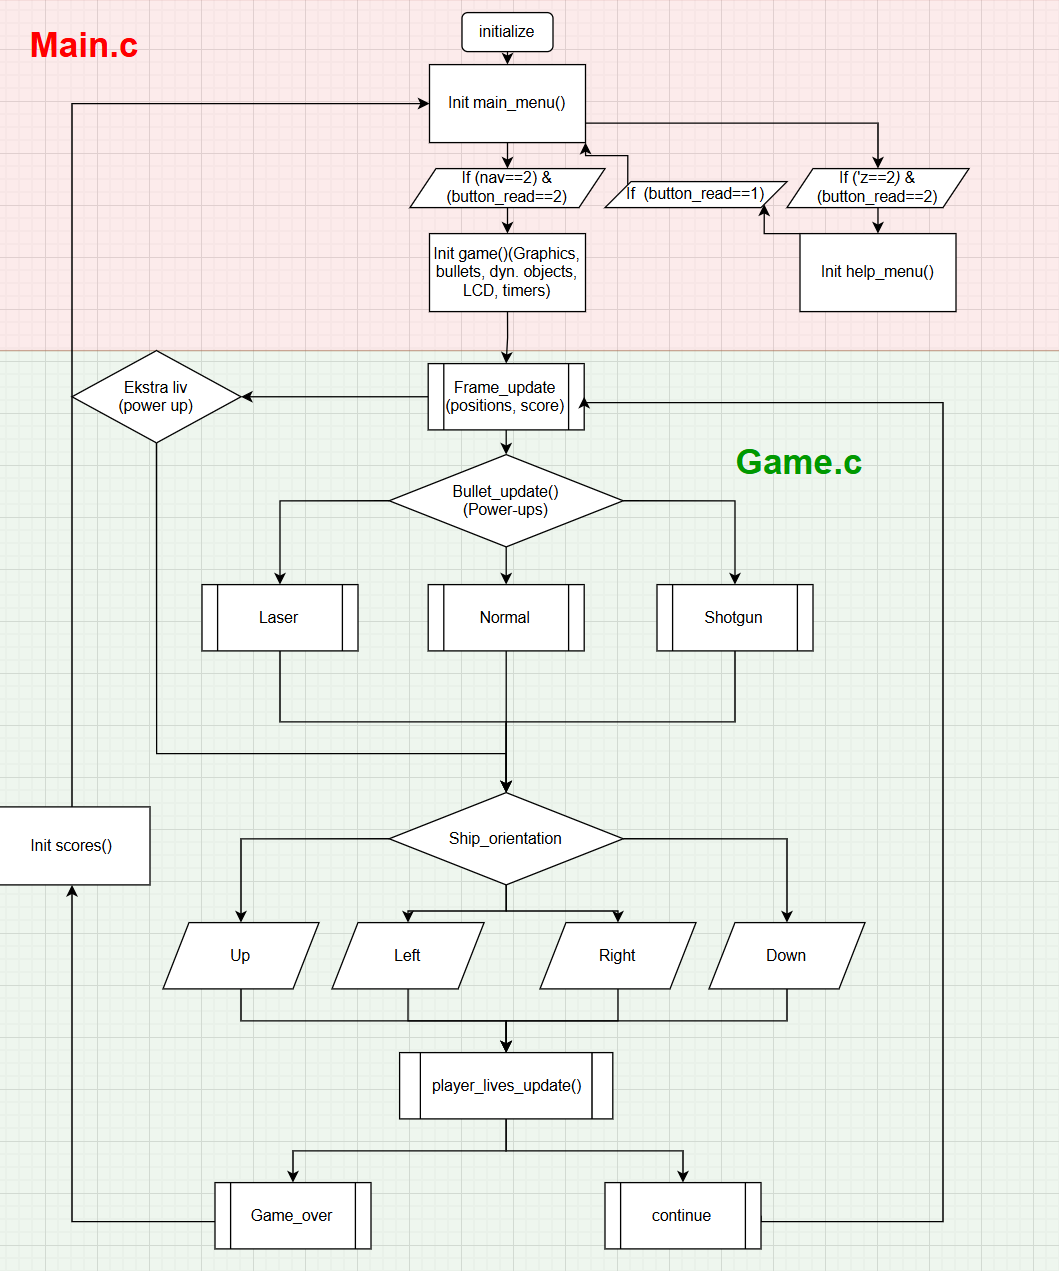
\includegraphics[width=0.75\linewidth]{figures/Main_flowchart.png}
    \caption{main.c flowchart}
    \label{fig:main_flowchart}
\end{figure}

\begin{figure}[H]
    \centering
    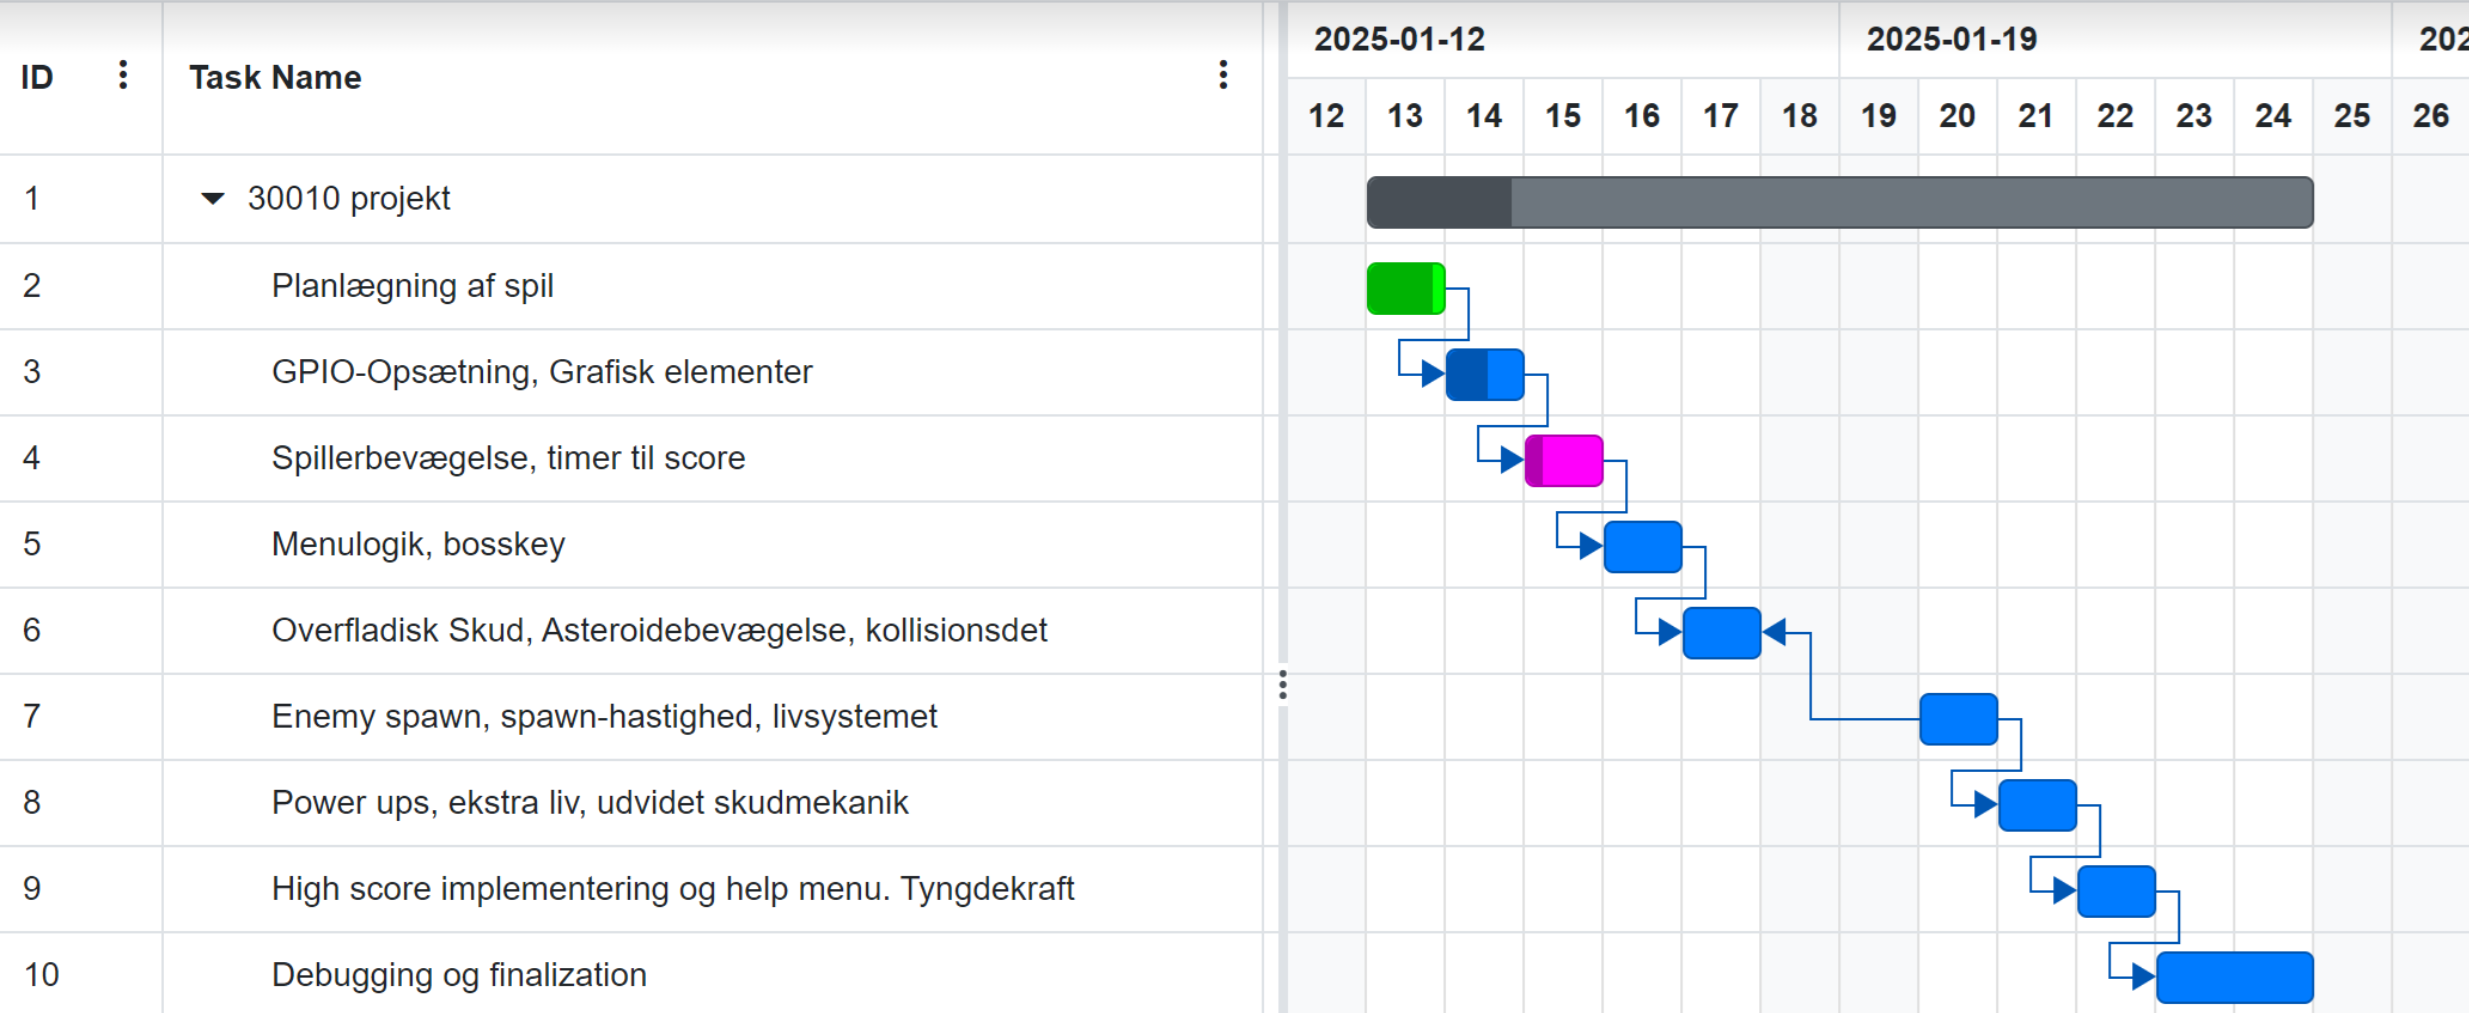
\includegraphics[width=1\linewidth]{figures/GANTT_30010.png}
    \caption{GANTT-chart}
    \label{fig:GANTT_chart}
\end{figure}
\begin{figure}
    \centering
    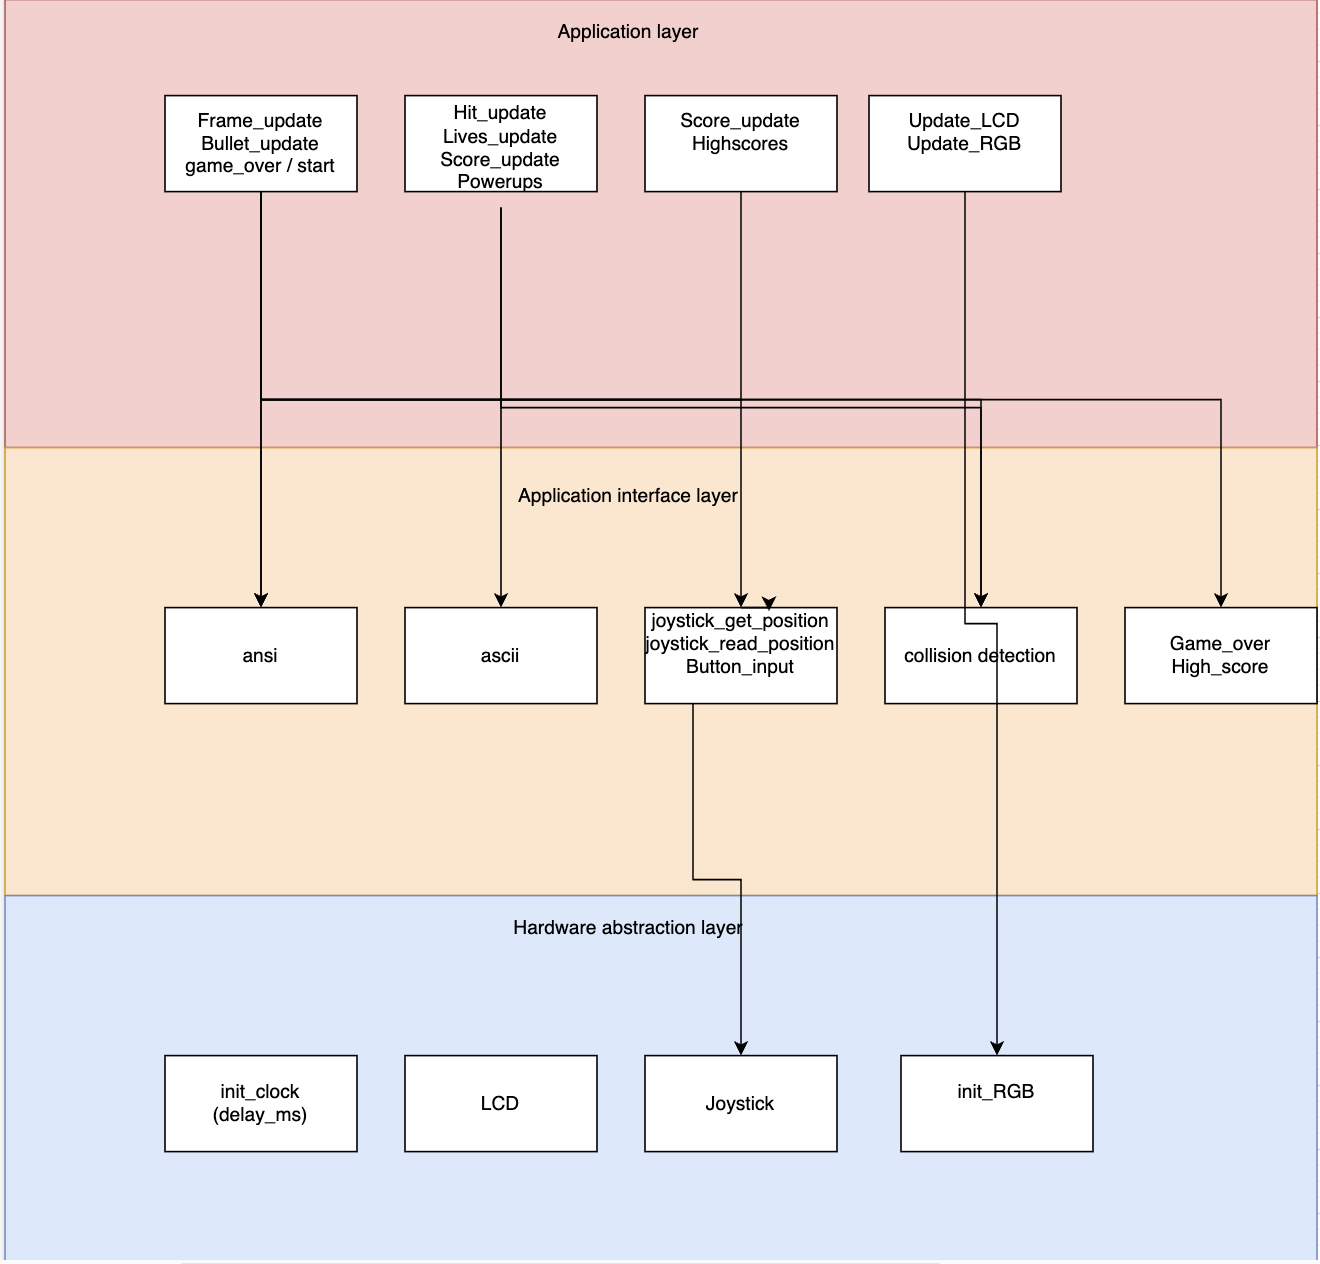
\includegraphics[width=0.5\linewidth]{figures/Block_diagram.png}
    \caption{Block diagram}
    \label{fig:block_diagram}
\end{figure}

\newpage
\label{kode:If-sætninger til normalt fungerende 30010 joystick}
\begin{lstlisting}[caption={If-sætninger til normalt fungerende 30010 joystick}] 
if ((1900 < x) && (x < 2100) && (1900 < y) && (y < 2100)) {
    new_value = 0;
} else if ((1900 < x) && (x < 2100) && (3700 < y) && (y < 4100)) {
    new_value = 8;
} else if ((3700 < x) && (x < 4100) && (1900 < y) && (y < 2100)) {
    new_value = 2;
} else if ((1900 < x) && (x < 2100) && (0 < y) && (y < 400)) {
    new_value = 4;
} else if ((0 < x) && (x < 400) && (1900 < y) && (y < 2100)) {
    new_value = 6;
} else if ((3000 < x) && (x < 3700) && (3000 < y) && (y < 3700)) {
    new_value = 1;
} else if ((3000 < x) && (x < 3700) && (300 < y) && (y < 1500)) {
    new_value = 3;
} else if ((200 < x) && (x < 1300) && (200 < y) && (y < 1300)) {
    new_value = 5;
} else if ((200 < x) && (x < 1300) && (3000 < y) && (y < 3700)) {
    new_value = 7;
}
\end{lstlisting}

\newpage
\pagenumbering{arabic}
\section{Appendiks B - Source Code} \label{ch11}
\input{Kode/Main.c} 
\input{Kode/ansi.ch}
\input{Kode/Background.ch}
\input{Kode/Boss_key.ch}
\input{Kode/Bullets.ch}
\input{Kode/Collision_detection.ch}
\input{Kode/Enemy.ch}
\input{Kode/Gamemenu.ch}
\input{Kode/Gamestart.ch}
\input{Kode/Gravity.ch}
\input{Kode/Helpmenu.ch}
\input{Kode/init_GPIO.ch}
\input{Kode/Joystick_reader.ch}
\input{Kode/LCD.ch}
\input{Kode/Led.ch}
\input{Kode/Mainmenu.ch}
\input{Kode/Movement.ch}
\input{Kode/Powerups.ch}
\input{Kode/Spaceship.ch}
\input{Kode/Spawn_powerups.ch}
\input{Kode/Timer.ch}
\input{Kode/Title.ch}


\newpage
\section{Appendix C - Exercise journal} \label{ch12}
\input{Journals/Journals}




\label{endOfDoc}
\end{document}
